\documentclass[11pt]{article}
\usepackage[letterpaper,margin=0.85in]{geometry}
\usepackage[hidelinks]{hyperref}
\usepackage{enumitem}
\usepackage{titlesec}
\usepackage{tabularx}
\usepackage{graphicx}

\setlist[itemize]{leftmargin=1.2em,itemsep=3pt,topsep=3pt}
\titleformat{\section}{\large\bfseries}{}{0em}{}[\titlerule]

\newcommand{\entry}[4]{
  \noindent\begin{tabularx}{\textwidth}{@{}Xr@{}}
    \textbf{#1} & #2 \\
    \textit{#3} & \textit{#4}
  \end{tabularx}\vspace{2pt}
}

\begin{document}

\noindent\begin{minipage}[t]{0.76\textwidth}
\vspace{0pt}
{\LARGE \textbf{Piter Z. Garcia Bautista}}\\[4pt]
Rochester, NY \textbar\ +1 (646) 288-3300 \textbar\ \href{mailto:pzg8794@rit.edu}{pzg8794@rit.edu} \textbar\ \href{mailto:pitergarcia@rochester.edu}{pitergarcia@rochester.edu}\\
\href{https://linkedin.com/in/garciapiterz}{linkedin.com/in/garciapiterz} \textbar\
\href{https://github.com/pzg8794}{github.com/pzg8794} \textbar\
\href{https://garciapiterz.com}{garciapiterz.com}
\end{minipage}%
\hfill\begin{minipage}[t]{0.20\textwidth}
\vspace{0pt}
\raggedleft
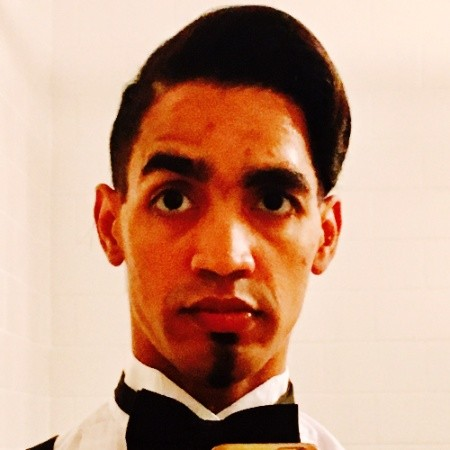
\includegraphics[width=\linewidth]{profile_pic}
\end{minipage}
\vspace{6pt}

\section{Research Profile}
Graduate researcher and NSF Robert Noyce Scholar working at the intersection of quantum computing, compiler-level optimization, and reproducible experimentation. Current research spans quantum network optimization, fault-tolerant routing, and fairness-aware decision workflows. Specifically interested in compiler-assisted precision and resource management for fault-tolerant quantum workloads, as explored in the SPQR project and TAFFO-inspired frameworks for quantum error correction code selection.

\section{Research Interests}
Quantum compiler optimization and error correction code selection; fault-tolerant quantum circuit design; LLVM/MLIR-based compiler backends for quantum workloads; reproducible benchmarking and structured experimental design; quantum-classical hybrid methods.

\section{Education}

\entry{Rochester Institute of Technology}{Expected Aug 2026}{Master of Science, Data Science --- GPA 3.9}{Rochester, NY}
\begin{itemize}
  \item Concentration: Bioinformatics \& Artificial Intelligence.
  \item Relevant coursework: Foundations of Data Science (DSCI-633), Software Engineering for Data Science (DSCI-644), Applied Data Science I (DSCI-601), Bioinformatics Algorithms (BIOL-630), Data-Driven Knowledge Discovery (ISTE-780).
\end{itemize}

\entry{University of Rochester, Warner School of Education}{Expected Aug 2026}{Master of Science track, Teaching Computer Science K--12 --- GPA 4.0}{Rochester, NY}
\begin{itemize}
  \item NSF Robert Noyce Teacher Scholarship Program (\$30,000 full funding).
  \item Advanced Certificate in Leadership in Disability and Inclusive Practices.
\end{itemize}

\entry{Rochester Institute of Technology}{2015}{Master of Science, Computer Science --- GPA 3.2}{Rochester, NY}
\begin{itemize}
  \item Concentrations: Computer Graphics, Artificial Intelligence, Big Data Analytics.
  \item Coursework in compiler design, algorithm analysis, and distributed systems.
\end{itemize}

\entry{Farmingdale State College}{2012}{Bachelor of Science, Computer Engineering Technology --- GPA 3.3}{Farmingdale, NY}
\begin{itemize}
  \item Dual degree: Electrical Engineering \& Computer Engineering Technology.
  \item Honors: CSTEP Award \& Merit, Dual BS Scholarship.
\end{itemize}

\section{Research and Professional Experience}

\entry{Rochester Institute of Technology}{Fall 2025 -- Present}{Graduate Assistant, Quantum and AI Research}{Rochester, NY}
\begin{itemize}
  \item Conduct research on quantum network path optimization and fault-tolerant routing under adversarial and stochastic conditions.
  \item Develop compiler-level experimental infrastructure for quantum circuit workloads using Qiskit and Cirq.
  \item Implement and validate quantum error correction code selection workflows in simulation (Stim-compatible pipelines).
  \item Apply LLVM/MLIR IR-level analysis concepts to quantum compilation pipeline studies; reviewed TAFFO precision-tuning methodology for applicability to quantum resource management.
\end{itemize}

\entry{University of Rochester, Warner School of Education}{Sep 2024 -- Present}{CS Teacher Candidate \& Education Research (NSF Noyce Scholar)}{Rochester, NY}
\begin{itemize}
  \item Deliver K--12 computer science instruction in active public school placement as part of the NSF Robert Noyce Scholar program, including computational thinking, inclusive pedagogy, and NYS learning standards.
  \item Conduct applied education research on AI-informed and data-driven approaches to improve learning outcomes for neurodivergent students, applying Universal Design for Learning (UDL) and evidence-based adaptive strategies.
  \item Produce lesson artifacts and instructional analyses documenting the intersection of AI, inclusive education, and evidence-based CS pedagogy.
\end{itemize}

\entry{VEDADATA Inc.}{Sep 2022 -- Aug 2024}{Data Solutions Engineer}{New York, NY}
\begin{itemize}
  \item Designed scalable Python workflows for ingestion, validation, and statistical diagnostics, emphasizing data reliability and structured quality checks.
  \item Strengthened production reliability through anomaly detection, schema validation, and structured logging.
\end{itemize}

\entry{VIOME Inc.}{Jan 2021 -- Sep 2022}{AI Data Solutions Engineer}{New York, NY}
\begin{itemize}
  \item Developed healthcare ML workflows for feature engineering, model experimentation, and reliability-aware evaluation in AWS-based production environments.
  \item Implemented uncertainty-quantification and model-monitoring components to flag prediction instability under distribution shift.
\end{itemize}

\section{Selected Technical Writing}
\begin{itemize}
  \item \textit{Quantum Network Path Optimization and Fault-Tolerant Routing} (manuscript under review, 2025--2026) --- quantum-classical hybrid ML for fault-tolerant routing under noise constraints and decoherence.
  \item \textit{Big Data Medical Diagnosis: A Multi-Method Approach} (RIT M.S.\ Computer Science graduate research, 2015) --- ensemble and deep learning methods for clinical classification on high-dimensional biomedical data.
  \item \textit{Predicting Hospital Readmission Rates: A Multi-Method ML Analysis} (DSCI-633 Project Report, 2025) --- ensemble and regularized regression methods for clinical risk stratification under distribution shift.
  \item \textit{BIO614-FinalProjectProposal} (Overleaf manuscript, 2026) --- RNA secondary structure prediction with thermodynamic deep learning enhancements, reproducible benchmarking, and biological interpretation.
  \item \textit{Equitable Bioinformatics: Enhancing Diagnostic Decision-Making through RNA and Biomarker Data} (ISTE-780 Project Report, 2025) --- fairness-aware ML for genomic diagnostic algorithms with SHAP-based bias detection and statistical significance testing.
  \item \textit{Differential Gene Expression in Murine DRG Neurons Following Sciatic Nerve Injury: An NGS Reanalysis} (BIOL550 Computational Biology Project, 2026) --- reproducible bulk RNA-seq pipeline using DESeq2, QC validation, and pathway-level biological interpretation of nociceptor gene expression.
  \item \textit{Fairness-Aware Bandits for Clinical Decision Systems} (DSCI-601 Project Proposal, 2025) --- bandit learning with equity constraints applied to high-stakes clinical diagnostic decision-making, addressing demographic disparity in sequential clinical recommendation workflows.
\end{itemize}

\section{Awards \& Recognition}
\begin{itemize}
  \item NSF Robert Noyce Teacher Scholarship (2024--2026) --- full funding for M.S.\ in Teaching Computer Science K--12.
  \item MS International Scholarship (2012--2015) --- MESCYT \& RIT, awarded for academic excellence.
  \item Honorable Mention Technology Award (2012) --- NYS STEP/CSTEP, 2nd place capstone project.
  \item IEEE Alumni Member (2009--Present) --- Member No.\ 90613000.
\end{itemize}

\section{Technical Competencies}
\textbf{Programming:} Python, R, Java, C++, C\#, MATLAB, SQL, JavaScript, Bash\\
\textbf{Quantum Computing:} Qiskit, Cirq (gate-based quantum circuit simulation and algorithm development)\\
\textbf{Compiler \& Systems:} LLVM/MLIR compiler backend framework; TAFFO/Precimonious (approximate computing and precision tuning)\\
\textbf{Machine Learning:} PyTorch, TensorFlow, scikit-learn, XGBoost, fairness-aware ML, contextual bandit workflows\\
\textbf{Data \& Analysis:} pandas, NumPy, SciPy, SHAP analysis, statistical testing, reproducible benchmarking\\
\textbf{Infrastructure:} AWS, GCP, Docker, Git/GitHub, Linux, LaTeX

\section{Selected Fit for NTNU Quantum Compiler Technologies Position}
\begin{itemize}
  \item Directly relevant research in quantum circuit optimization and fault-tolerant routing; active study of compiler-assisted precision tuning methodologies (TAFFO, Precimonious) and their extension to QEC code selection.
  \item Hands-on experience with LLVM/MLIR IR-level analysis and quantum circuit frameworks (Qiskit, Cirq) providing a practical foundation for compiler backend contributions within the SPQR project.
  \item Reproducibility-first experimental discipline (multi-environment: local, Colab, GCP) with traceable infrastructure---well matched to SSG's open-source and benchmark-driven research culture (CGO, PLDI).
  \item Interest in PoliMi collaboration; familiar with TAFFO's Value Range Analysis approach as the classical precedent the SPQR project extends to the quantum domain.
\end{itemize}

\end{document}
